%
% chapter.tex
%
% (c) 2020 Prof Dr Andreas Müller
%
\chapter{Partielle Differentialgleichungen\label{chapter:pde}}
\lhead{Partielle Differentialgleichungen}
\rhead{}
Elektrische oder magnetische Felder sind Funktionen der Ortskoordinaten
und der Zeit.
\index{Feld}%
\index{elektrisch}%
\index{magnetisch}%
\index{Ladung}%
\index{Maxwellsche Gleichungen}%
Die Veränderung dieser Felder mit der Zeit hängt ab von der Anwesenheit
oder der Bewegung von Ladungen, wie sie von den Maxwellschen Gleichungen
\index{nabla@$\nabla$}%
\begin{align*}
\nabla\cdot\vec{E} &= \frac{\varrho}{\varepsilon_0}
\\
\nabla\cdot\vec{B} &= 0
\\
\nabla\times\vec{E} &= -\frac{\partial\vec{B}}{\partial t}
\\
\nabla\times\vec{B} &= \mu_0\vec{\jmath}
	+ \frac{1}{c^2}\frac{\partial\vec{E}}{\partial t}
\end{align*}
beschrieben werden.
Diese Gleichungen zwischen den Komponenten der Felder enthalten
die partiellen Ableitungen der gesuchten Funktionen nach Ortskoordinaten
und der Zeit.
\index{partielle Differentialgleichung}
\index{Differentialgleichung!partiell}
Solche {\em partiellen Differentialgleichungen} können nicht mit den Methoden
gelöst werden, die für gewöhnliche Differentialgleichungen entwickelt 
worden sind.
In diesem Kapitel sollen die wichtigsten Ideen zusammengetragen werden,
die besser geeigneten Verfahren zu Grunde liegen.

%
% problem.tex
%
% (c) 2020 Prof Dr Andreas Müller, Hochschule Rapperswil
%
\section{Problemstellung
\label{section:pde:problem}}
\rhead{Problemstellung}
\index{Differentialgleichung!gewöhnlich}%
\index{gewöhnliche Differentialgleichung}%
Gewöhnliche Differentialgleichungen werden durch eine einzige Funktion
$f\colon \mathbb R\times\mathbb R^n: (t,x)\mapsto f(t,x)$ beschrieben,
werden.
Eine Lösung der Differentialgleichung
\begin{equation}
\frac{dx}{dt} = f(t,x)
\label{pde:eqn:ode}
\end{equation}
mit der Anfangsbedingung
\[
x(t_0) = x_0
\]
ist eine Funktion $x(t)$ mit $x(t_0)=x_0$ derart, dass 
\[
\frac{dx(t)}{dt} = f(t, x(t)).
\]
Das Definitionsgebiet der Lösungsfunktion $x(t)$ ist ein Intervall
der Form $[t_0,a]$ mit $a>t_0$.
\index{Definitionsgebiet}%

Für eine partielle Differentialgleichung ist die Situation wesentlich
komplizierter.
Zunächst gibt es Ableitungen der gesuchten Funktion $u(x_1,\dots,x_n)$
nach allen unabhängigen Variablen zu
berücksichtigen, so dass eine explizite Form der Differentialgleichung
wie in~\eqref{pde:eqn:ode} grundsätzlich nicht mehr möglich ist.
Das Definitionsgebiet ist eine fast beliebige Teilmenge
$\Omega\subset\mathbb R^n$ eines $n$-dimensionalen Raumes.
Insbesondere kann das Definitionsgebiet sehr viel komplizierter sein
als im Falle einer gewöhnlichen Differentialgleichungen.
Die Form des Gebietes hat einen wesentlichen Einfluss auf die Lösungen
der Differentialgleichung.
Schliesslich wird es nicht mehr genügen, Werte in nur einem Randpunkt
des Gebietes zu kennen, wie das bei einer gewöhnlichen Differentialgleichung
der Fall war.
Vielmehr ist es eine nichttriviale Frage, auf welchem Teil des Randes
$\partial\Omega$ von $\Omega$ welche Funktions- oder Ableitungswerte
vorgegeben werden müssen, damit die Lösung der Differentialgleichung
eindeutig bestimmt ist.

Der Einfachheit halber betrachten wir in diesem Kapitel nur partielle
Differentialgleichungen für eine skalare Funktion $u=u(x_1,\dots,x_n)$.
In diesem Abschnitt geht es darum zu klären, wie genau ein solches
Problem gestellt werden muss.
In Abschnitt~\ref{subsection:pde:gebiet} studieren wir ein sinnvolles
Definitionsgebiet für die Differentialgleichung.
In Abschnitt~\ref{subsection:pde:klassifikation} klassifizieren wir
mögliche Differentialgleichungen bevor wir in
Abschnitt~\ref{subsection:pde:randbedingungen} Randbedingungen und
in Abschnitt~\ref{subsection:pde:loesungen} Lösungen beschreiben.

\subsection{Gebiet und Rand
\label{subsection:pde:gebiet}}
Eine partielle Differentialgleichung sucht eine Funktion
\index{partielle Differentialgleichung}%
\index{Differentialgleichung!partiell}%
\[
u\colon \Omega\to\mathbb R
\]
$u(x_1,\dots,x_n)$, für die Beziehungen zwischen den partiellen
Ableitungen nach den unabhängigen Variablen gelten.
Für alle Punkte einer Menge $\Omega\subset\mathbb R^n$ muss
als eine Gleichung ähnlich wie zum Beispiel
\[
\Delta u
=
\frac{\partial^2 u}{\partial x_1^2}
+
\dots
+
\frac{\partial^2 u}{\partial x_n^2}
=
0
\qquad
\forall \;
(x_1,\dots,x_n)\in \Omega
\]
gelten, $\Delta$ ist der {\em Laplace-Operator}.
\index{Laplace-Operator}%
Diese Beobachtung schränkt die Art der Menge $\Omega$ bereits ein,
wie im Folgenden diskutiert werden soll.

\begin{figure}
\centering
\includegraphics{chapters/70-pde/images/offen.pdf}
\caption{Jeder innere Punkt einer Menge hat eine $\varepsilon$-Umgebung, 
die ebenfalls in der Menge enthalten ist.
Jede Umgebung des Punktes $P$ enthält aber auch Punkte ausserhalb der
Menge $\Omega$, $P$ ist daher ein Randpunkt.
\label{buch:pde:figure:offen}}
\end{figure}

Die Ableitung einer Funktion $u(x_1,\dots,x_n)$ in einem Punkt
$x_0=(x_{0,1},\dots,x_{0,n})$ ist eine lineare Funktion 
$Du(x_{0,1},\dots,x_{0,n}) $ derart, dass
\[
u(x_1,\dots,x_n) - u(x_{0,1},\dots,u_{0,n})
=
Du(x_{0,1},\dots,x_{0,n})\cdot (x-x_0) + o(|x-x_0|).
\]
Das Symbol $o(|x-x_0|)$ beschreibt eine Funktion, die schneller als
ihr Argument gegen $0$ geht, so dass für den Grenzwert des
Quotienten 
\[
\lim_{x\to x_0}\frac{o(|x-x_0|)}{|x-x_0|} = 0
\]
gilt.
Der Grenzwert bedeutet, dass es für jedes $\varepsilon>0$ eine Umgebung
\index{Umgebung}%
$U_\delta(x_0)=\{x\;|\; |x-x_0|<\delta\}$ gibt derart, dass
\index{Udeltax0@$U_\delta(x_0)$}
\[
\bigl|
u(x)-u(x_0) - Du(x_0)\cdot (x-x_0)
\bigr|
< \varepsilon\cdot |x-x_0|
\qquad\forall x\in U_\delta(x_0)
\]
ist.
Dies ist nur sinnvoll, wenn die ganze Umgebung $U_{\delta}(x_0)\subset \Omega$
im Definitionsgebiet $\Omega$ der Differentialgleichung vorhanden ist.
Dies führt auf die folgende Definition (siehe auch Abbildung~\ref{buch:pde:figure:offen}.

\begin{definition}
\index{offene Menge}%
\index{Gebiet}%
\index{Menge!offen}%
Eine Menge $\Omega$ heisst {\em offen}, wenn mit jedem Punkt $x\in \Omega$
auch eine offene Umgebung $U_{\delta}(x)\subset\Omega$ darin enthalten ist.
Ein {\em Gebiet} ist eine offene Menge in $\mathbb R^n$.
\end{definition}

Gebiete sind also genau die sinnvollen Definitionsgebiete für eine partielle
Differentialgleichung.
\index{Definitionsgebiet}%
Es reicht allerdings nicht, dass die Funktion $u$ auf $\Omega$ definiert
ist, da ja auch noch Randwerte erfüllt werden müssen.

\begin{figure}
\centering
\includegraphics{chapters/70-pde/images/gebiet.pdf}
\caption{Inneres und Rand einer Punktmenge $A$ in der Ebene.
Die sechs Strahlen der Menge $A$ links können nichts zu den Randwerten
einer partiellen Differentialgleichunb beitragen, weil sie keinen
Einfluss auf Werte in inneren Punkten (Mitte) haben können.
\index{Strahlen}%
Randwerte müssen daher nur auf einem Teil des Randes $\partial\mathring{A}$
des Inneren (rechts) spezifiziert werden.
\label{buch:pde:figure:gebiet}}
\end{figure}

\begin{definition}
Der {\em Abschluss} $\bar{\Omega}$ einer Menge $\Omega\subset\mathbb R^n$ ist
die Menge aller Punkte in $\mathbb R^n$, die Grenzwerte von Folgen in
$\Omega$ sind.
\index{Abschluss}%
Das {\em Innere} $\mathring{A}$ einer Menge $A$ ist die Menge aller Punkte
$x$ derart, dass es eine Umgebung $U_\delta(x)$ gibt, die ganz in $A$
enthalten ist: $U_{\delta}(x)\subset A$.
\index{Inneres}%
\end{definition}

Alternativ kann man den Abschluss auch charakterisieren als die Menge
aller Punkte $x\in\mathbb R^n$, für die jede beliebige Umgebung
$U_\delta(x)$ auch Punkte von $\Omega$ enthält, also
$U_\delta(x)\cap \Omega\ne \emptyset$.
Ein Gebiet ist offen, daher ist $\mathring\Omega=\Omega$.

Die Lösung einer partiellen Differentialgleichung wird im Allgemeinen erst
festgelegt sein, wenn zusätzlich Werte auf Teilen des ``Randes'' des
Gebietes festgelegt worden sind.
Nur Punkte, die als Grenzwerte von Punkten in $\Omega$ erreicht werden
können, können zu diesem Zweck hinzugezogen werden.

\begin{definition}
Der {\em Rand} $\partial A$ einer Menge $A\subset\mathbb R^n$ ist
$\partial A=\bar{A}\setminus\mathring{A}$.
\index{Rand}
\index{d@$\partial A$}
\end{definition}

Während also eine Differentialgleichung typischerweise auf einem
Gebiet $\Omega$ definiert ist, muss die gesuchte Lösungsfunktion
sogar auf auf dem Abschluss $\bar{\Omega}$ definiert sein.
Die Lösung wird im Allgemeinen erst dadurch festgelegt, dass zusätzlich
Werte oder Ableitungen auf Teilen des Randes $\partial\Omega$ 
vorgegeben werden.

\subsection{Klassifikation der partiellen Differentialgleichungen
\label{subsection:pde:klassifikation}}
Eine partielle Differentialgleichung beschreibt eine Beziehung 
zwischen den partiellen Ableitungen der Funktion $u(x_1,\dots,x_n)$.
Dies ist auf sehr vielfältige Arten möglich, in die dieser Abschnitt
etwas Ordnung bringen soll.

\subsubsection{Ordnung}
Wie bei den gewöhnlichen Differentialgleichungen klassifizieren wir
auch partielle Differentialgleichungen nach der Ordnung.
\index{Ordnung!einer partiellen Differentialgleichung}%
\index{partielle Differentialgleichung!Ordnung}

\begin{definition}
Die {\em Ordnung} einer partiellen Differentialgleichung ist die
Ordnung der höchsten Ableitung, die in der Differentialgleichung
vorkommt.
\index{Ordnung}%
\end{definition}

Für die folgende Diskussion reicht es, partielle Differentialgleichungen
zweiter Ordnung zu betrachten.
Die meisten in den Anwendungen vorkommenden Differentialgleichungen
sind von dieser Art, so dass dies eine unwesentliche Einschränkung ist.
Die Erweiterungen für höhere Ordnung sind offensichtlich.

\subsubsection{Linearität}
Die Beziehung zwischen den Ableitungen kann beschrieben werden durch
eine Funktion
\[
F(x_1,\dots,x_n,u,p_1,\dots,p_n,t_{11},t_{12},\dots,t_{nn})
\]
derart, dass nach der Substitution
\begin{align*}
u&\to u(x_1,\dots,x_n)
\\
p_i&\to \frac{\partial u}{\partial x_i}
\\
t_{ij} &Ò\to \frac{\partial^2 u}{\partial x_i\,\partial x_j}
\end{align*}
die Differentialgleichung
\[
F\biggl(
x_1,\dots,x_n,u(x_1,\dots,x_n),
\frac{\partial u}{\partial x_1},\dots,\frac{\partial u}{\partial x_n},
\frac{\partial^2u}{\partial x_1^2},
\frac{\partial^2u}{\partial x_1\,\partial x_2},\dots,
\frac{\partial^2u}{\partial x_n^2}
\biggr)
=0
\]
entsteht.
Für höhere Ordnung werden weitere Variablen benötigt, die für die
höheren Ableitungen stehen.
Die Funktion $F$ kann also dazu verwendet werden, die verschiedenen
möglichen partiellen Differentialgleichungen zu klassifizieren.

Eine partielle Differentialgleichung heisst {\em linear}, wenn die
Funktion $F$ linear ist in den Argumenten $u$, $p_i$ und $t_{ij}$,
wenn also gilt
\begin{align}
F(\dots,\lambda u' + \mu u'',\dots)
&=
\lambda F(\dots,u',\dots) + \mu F(\dots,u'',\dots)
\label{pde:eqn:linearu}
\\
F(\dots,\lambda p'_i+\mu p''_i,\dots)
&=
\lambda F(\dots,p'_i,\dots) + \mu F(\dots,p''_i,\dots)
&&\forall i
\label{pde:eqn:linearp}
\\
F(\dots,\lambda t'_{ij}+\mu t''_{ij},\dots)
&=
\lambda F(\dots,t'_{ij},\dots) + \mu F(\dots,t''_{ij},\dots)
&&\forall i,j.
\label{pde:eqn:lineart}
\end{align}
Eine partielle Differentialgleichung heisst {\em quasilinear}, 
wenn die Funktion $F$ linear ist in den Argumenten $p_i$ und $t_{ij}$,
wenn also die Bedingungen~\eqref{pde:eqn:linearp} und \eqref{pde:eqn:lineart}
gelten.
\index{quasilinear}%
Linearität in $u$, also die Bedingung~\eqref{pde:eqn:linearu} ist
für eine quasilineare partielle Differentialgleichung nicht verlangt.

\begin{beispiel}
Die Differentialgleichung
\[
\frac{\partial^2 u}{\partial x_1^2}
+
\frac{\partial^2 u}{\partial x_2^2}
=
0
\]
zweiter Ordnung wird beschrieben durch die Funktion
\[
F(x_1,x_2,u,p_1,p_2,t_{11},t_{12},t_{22})
=
t_{11} + t_{22}.
\]
Diese Funktion ist linear in $t_{11}$ und $t_{22}$.
\end{beispiel}

\begin{beispiel}
Die partielle Differentialgleichung erster Ordnung von Burgers
(Siehe auch Kapitel~\ref{chapter:burgers})
\index{Burgers}%
\index{Gleichung!von Burgers}%
\begin{equation}
\frac{\partial u}{\partial x_1}
+
u
\frac{\partial u}{\partial x_2}
=
0
\label{buch:eqn:burgers}
\end{equation}
wird beschrieben durch die Funktion
\[
F(x_1,x_2,u,p_1,p_2)
=
p_1+up_2.
\]
Diese Funktion ist nicht linear in $u$ und $p_2$, aber linear in
$p_1$ und $p_2$.
\eqref{buch:eqn:burgers} ist also eine quasilineare partielle
Differentialgleichung.
\end{beispiel}

\subsubsection{Lineare Differentialgleichungen zweiter Ordnung}
Ein für die Anwendungen besonders wichtiger Fall sind lineare
Differentialgleichungen zweiter Ordnung.
Für eine solche Gleichung ist die Funktion $F$ immer von der Form
\[
F(x_i,u,p_i,t_{ij})
=
\sum_{i,j=1}^n a_{ij}(x_1,\dots,x_n)t_{ij} + \sum_{i=1}^n b_i(x_1,\dots,x_n) p_i + c(x_1,\dots,x_n) u 
\]
Die Koeffizienten $a_{ij}$, $b_i$ und $c$ dürfen also von den Variablen
$x_1,\dots,x_n$ abhängen, nicht aber von $u$ oder den Ableitungen.
Die Differentialgleichung hat also die Form
\begin{equation}
\sum_{i,j=1}^n
a_{ij}\frac{\partial^2 u}{\partial x_i\,\partial x_j}
+
\sum_{i=1}^n
b_i\frac{\partial u}{\partial x_i}
+
cu
=
f
\label{pde:eqn:eqn2nd}
\end{equation}
Da es in den zweiten Ableitungen nicht auf die Reihenfolge ankommt,
kann die Matrix $a_{ij}$ immer symmetrisch gewählt werden.
Die Matrix $A=(a_{ij})$ heisst die {\em Symbolmatrix} der Differentialgleichung.
\index{Symbolmatrix}%

Es stellt sich heraus, dass die Terme zweiter Ordnung, also die 
Matrix $A$, das Verhalten der Lösung wesentlich beeinflussen.
Eine symmetrische Matrix kann durch eine Drehung immer in eine
Diagonalmatrix transformiert werden.
Durch Wechsel des Koordinatensystems kann man also erreichen, dass
\[
A
=
\begin{pmatrix}
\lambda_1&         &      &         \\
         &\lambda_2&      &         \\
         &         &\ddots&         \\
         &         &      &\lambda_n
\end{pmatrix}
\]
ist.
In diesen Koordinaten sind es nur noch die Eigenwerte
$\lambda_1,\dots,\lambda_n$ der Matrix $A$, die das Verhalten der Lösung
bestimmen.

\begin{definition}
Die Differentialgleichung
\eqref{pde:eqn:eqn2nd}
heisst {\em elliptisch}, wenn alle Eigenwerte positiv sind.
Sie heisst {\em hyperbolisch}, wenn alle Eigenwerte bis auf einen negativen
positiv sind.
Sie heisst {\em parabolisch}, wenn alle Eigenwerte bis auf einen
verschwindenden positiv sind.
\end{definition}
\index{elliptische partielle Differentialgleichung}%
\index{elliptisch}%
\index{hyperbolische partielle Differentialgleichung}%
\index{hyperbolisch}%
\index{parabolische partielle Differentialgleichung}%
\index{parabolisch}%

\begin{beispiel}
Die {\em Wellengleichung}
\index{Wellengleichung}%
\[
\frac{1}{a^2}\frac{\partial^2 u}{\partial t^2}
=
\Delta u 
\quad\Rightarrow\quad
\Delta u 
-
\frac{1}{a^2}\frac{\partial^2 u}{\partial t^2}
=
0
\]
hat die Symbolmatrix
\[
A=
\begin{pmatrix}
1& &      &              \\
 &1&      &              \\
 & &\ddots&              \\
 & &      &\displaystyle-\frac{1}{a^2}
\end{pmatrix}
\]
$n$ positive und einem negativen Eigenwert, diese Gleichung ist also
hyperbolisch.
Die Lösungen zeigen Wellencharakter und die Werte und ersten
Ableitungen von $u$ zu einem Zeitpunkt $t_0$ bestimmen das Verhalten
der Lösung vollständig.
Eine hyperbolische Differentialgleichung hat also eine natürlich
``Entwicklungsrichtung'', das Gebiet kann in Richtung ``Zukunft''
offen sein, ohne dass die Eindeutigikeit der Lösung dadurch gefährdet wird.
\end{beispiel}

\begin{beispiel}
Die Gleichung für das Potential einer Ladungsverteilung
\index{Ladungsverteilung}%
\[
\Delta u = f
\qquad\Rightarrow\qquad
A=
\begin{pmatrix}
1& &      & \\
 &1&      & \\
 & &\ddots& \\
 & &      &1
\end{pmatrix}
=E
\]
hat nur positive Eigenwerte, sie ist also elliptisch.
Die Lösungen dieser Gleichung sind nur dann bestimmt, wenn Werte von $u$
auf dem gesamten Rand des Gebietes vorgegeben werden.
Es ist also nicht möglich, eine ``Zeitrichtung'' für die Entwicklung
der Lösung einer solchen Differentialgleichung zu finden.
\index{Zeitrichtung}%
\end{beispiel}

Die Verschiedenartigkeit der Lösungen in Abhängigkeit vom Typ der
Differentialgleichung hat zur Folge, dass verschiedene Lösungsverfahren
zum Einsatz kommen müssen.
Die Klassifikation einer Differentialgleichung ist also Vorbedingung
für die Wahl eines geeigneten Lösungsverfahrens.
\index{Klassifikation!partielle Differentialgleichung}

\subsection{Randbedingungen
\label{subsection:pde:randbedingungen}}
Die Lösung einer partiellen Differentialgleichung ist erst eindeutig
bestimmt, wenn Werte von $u$ oder von Ableitungen von $u$ auf geeignet
gewählten Teilen das Randes $\partial\Omega$ des Gebietes $\Omega$
vorgegeben sind.
Die Theorie der partiellen Differentialgleichungen studiert ausführlich,
welche Art von Randbedingungen wo auf dem Rand zu spezifizieren sind.
\index{Randbedingung}%

\subsubsection{Dirichlet-Randbedingungen}
Werte der Funktion auf dem Rand können vorgegeben werden, indem eine
Funktion $g\colon \partial\Omega\to\mathbb R$ spezifiziert wird, so
dass für alle Punkte $x\in\partial\Omega$ die Gleichung
$
u(x) = g(x) 
$
gilt.
Diese Art von Randbedingungen heisst {\em Dirichlet-Randbedingungen}.
\index{Dirichlet-Randbedingung}%
\index{Randbedingung!Dirichlet}%

\subsubsection{Neumann-Randbedingungen}
Die Theorie des Anfangswertproblems für gewöhnliche Differentialgleichungen
besagt, dass die Lösung einer Differentialgleichung $n$-ter Ordnung erst
festgelegt ist, wenn der Anfangswert und $n-1$-Ableitungen vorgegeben sind.
Es ist zu erwarten, dass es auch bei gewissen partiellen
Differentialgleichungen der Ordnung $n\ge 2$ nötig sein wird, 
Ableitungen auf dem Rand vorzugeben.

Im Allgemeinen wird es nicht genügen, nur Ableitungen vorzugeben,
da sie Funktionen nur bis auf eine Konstante festlegen können.
Es wird also nötig sind, mindestens in einem Punkt zusätzlich einen
Funktionswert vorzugeben.

Es ist jedoch nicht sinnvoll, beliebige Ableitungen auf dem Rand
vorzugeben.
Wir illustrieren dies an einem einfachen Beispiel.
Als Gebiet wählen wir $\Omega = \{(x,y)\in\mathbb R^2\;|\; x > 0\}$,
der Rand ist also die $y$-Achse.
Nehmen wir an, dass Werte der Ableitung $\partial u/\partial y$ 
auf der $y$-Achse vorgegeben sind, also
\[
\frac{\partial u}{\partial y}(0,y)  = g(y).
\]
Ausserdem nehmen wir an, dass der Funktionswert $u(0,0)=u_0$ vorgegeben ist.
Für die Funktion $f(y) = u(0,y)$ gilt daher $f'(y) = g(y)$ und $f(0)=u_0$.
Daraus lässt sich die Funktion $f$ aber durch das Integral
\[
f(y) = u_0 + \int_0^y g(\eta)\,d\eta
\]
bestimmen.
Die Vorgabe der Ableitung $\partial u/\partial y$ auf dem Rand und eines
Wertes ist also gleichbedeutend mit der Vorgabe aller Werte $f(y)$ auf dem
Rand.
Statt der Ableitungen $\partial u/\partial y$ hätten wird daher auch
Dirichlet-Randbedingungen $u(0,y) = f(y)$ vorgeben können.
Es ist also nur sinnvoll, die Ableitung $\partial u/\partial x$ 
auf dem Rand vorzugeben.

Weiter oben hat ein spezielles Beispiel bezeigt,
dass Ableitungen entlang des Randes gegenüber Dirichlet-Randbedingungen
keine neue Information liefern können.
Nur die Ableitung in die Richtung senkrecht auf den Rand kann zusätzliche
Information liefern.
Dazu muss der Rand des Gebietes ausreichend glatt sein, so dass die
Normale auf den Rand wohldefiniert ist.

\begin{definition}
Ist $u$ eine Funktion, die auf $\bar\Omega$ definiert ist.
Sei $n$ die Normale auf den Rand $\partial\Omega$ in einem Punkt
$x\in\partial\Omega$.
Die {\em Normalableitung}
\[
\frac{\partial u}{\partial n}
=
\lim_{t\to 0+} \frac{u(x+tn)-u(x)}{t}
\]
in $x$ ist die Richtungsableitung 
der Funktion $u$ in Richtung $n$.
\end{definition}
\index{Normalableitung}%

Im Falle der Wellengleichung
\[
\frac{\partial^2 u}{\partial x^2}
-
\frac{1}{a^2}
\frac{\partial^2 u}{\partial t^2}
=0
\]
beschreibt $u(t,x)$ zum Beispiel die Auslenkung einer gespannten Saite
aus der Ruhelage.
Es ist aus physikalischen Überlegungen klar, dass die Bewegung der Saite
erst dann festgelegt ist, wenn Auslenkung und Geschwindigkeit der Saite
zur Zeit $t=0$ vorgegeben werden.
Die Vorgabe der Auslenkung zur Zeit $t=0$
\[
u(0,x) = f(x)
\]
ist eine Dirichlet-Randbedingung.
Die Richtung $n$ der Zeitachse ist senkrecht auf dem Rand $t=0$,
die Zeitableitung von $u$ ist also genau eine Normalableitung.
Die Vorgabe der Geschwindigkeit
\[
\frac{\partial u}{\partial n}(0,x)
=
\frac{\partial u}{\partial t}(0,x)
=
g(x)
\]
ist also eine Vorgabe der Normalableitung.

\begin{definition}
Die Vorgabe der Normalableitung auf dem Rand $\partial\Omega$
\[
\frac{\partial u}{\partial n}(x) = h(x)\qquad \forall x\in\partial\Omega
\]
heisst eine {\em Neumann-Randbedingung}.
\end{definition}
\index{Neumann-Randbedingung}%
\index{Randbedingung!Neumann}%

\subsection{Lösungen
\label{subsection:pde:loesungen}}
Ein vollständig gestelltes Problem mit partiellen Differentialgleichungen
beginnt also immer mit einer Definition des Gebietes $\Omega$, also
einer offenen Menge in $\mathbb R^n$.
Die Differentialgleichung wird gegeben durch eine Funktion $F$ wie in
Abschnitt~\ref{subsection:pde:klassifikation} dargestellt.
Ausserdem müssen Randbedingungen vorgegeben werden, wie in
Abschnitt~\ref{subsection:pde:randbedingungen} dargestellt.
Gesucht ist dann eine Funktion $u$, welche alle diese Bedingungen
erfüllen soll.
Dazu muss die Funktion nicht nur in $\Omega$ definiert sein, 
sondern auch auf dem Rand.

\begin{definition}
Eine Lösung einer partiellen Differentialgleichung ist eine Funktion
\[
u\colon \bar{\Omega} \to \mathbb R:(x_1,\dots,x_n)\mapsto u(x_1,\dots,x_n)
\]
derart, dass die Differentialgleichung im Inneren, also in $\Omega$,
erfüllt ist, und die Randbedingungen auf $\partial\Omega$.
\end{definition}







%
% fdm.tex
%
% (c) 2020 Prof Dr Andreas Müller, Hochschule Rapperswil
%
\section{Finite Differenzen
\label{section:finite-differenzen}}
\rhead{Finite Differenzen}
Jedes Lösungsverfahren für partielle Differentialgleichungen muss die
unendlich vielen Freiheitsgrade, die eine Funktion
$u\colon\Omega\to\mathbb R$ enthalten kann, auf eine endlich Zahl von
Variablen reduzieren, für die sich ein Gleichungssystem aufstellen 
lässt, welches dann mit einer der früher studierten Methoden
gelöst werden kann.

%
% Gitter und Ableitungen
%
\subsection{Gitter und Ableitungen
\label{pde:subsection:gitter}}
Eine einfache Methode, die Funktion $u$ eine endliche Menge von Parametern
zu reduzieren, ist, nur die Werte in einzelnen Punkten des Gebietes 
$\Omega$ zu verwenden.
Als Beispiel betrachten wir ein Gebiet $\Omega\subset\mathbb R^2$
in der Ebene.
Dazu betrachten wir die Punkte
\[
x_{ik} = (ih_x, kh_y) \in \mathbb R^2
\qquad
i,k\in\mathbb Z,
\]
sie bilden ein Gitter $\Gamma$ mit Gitterkonstante oder Schrittweite
$h_x$ in $x$-Richtung und $h_y$ in $y$-Richtung.

Die Funktion $u(x,y)$ nimmt in den Punkten $x_{ik}$ die Werte
$u_{ik} = u(x_{ik})$ an.
Eine approximative Lösung der Differentialgleichung ist also
die Bestimmung der Werte $u_{ik}$ für die Punkte $x_{ik}$, die in
$\Omega$ liegen, für die also $x_{ik}\in\Omega$ gilt.
Dazu müssen jetzt die Randbedingungen und die Differentialgleichung
übersetzt werden in Gleichungen für die Unbekannten $u_{ik}$.

\subsubsection{Dirichlet-Randbedingungen}
Dirichlet-Randbedingungen geben die Werte auf dem Rand vor.
Liegt ein Punkt $x_{ik}$ des Gitters $\Gamma$ auf dem Rand $\partial\Omega$
von $\Omega$, dann geben die Dirichlet-Randbedingungen den Wert
dieser Variablen vor.
Es ist daher anzustreben, das Gitter $\Gamma$ so zu wählen, dass 
der Rand durch Gitterpunkte verläuft.
Ein gekrümmter Rand wird daher im Allgmeinen durch eine Kurve durch
die Gitterpunkte approximiert werden müssen.

\subsubsection{Erste Ableitungen}
\begin{figure}
\centering
\includegraphics{chapters/70-pde/images/derivatives.pdf}
\caption{Approximation der ersten Ableitung mit verschiedenen
Differenzausdrücken
\label{buch:pde:1abldiff}}
\end{figure}
Die naheliegenste Approximation für die Differentialgleichung besteht
darin, die Ableitungen durch Differenzenquotienten zu ersetzen (siehe 
Abbildung~\ref{buch:pde:1abldiff}).
Mit der oben eingeführten Notation können die ersten Ableitungen durch
die sogenannten {\em Vorwärtsdifferenzen}
\index{Vorwärtsdifferenz}%
\begin{align}
\frac{\partial u}{\partial x} (x_{ik}) 
&\simeq
\frac{u(x_{i+1,k}) - u(x_{ik})}{h_x}
&
&\text{und}
&
\frac{\partial u}{\partial y} (x_{ik}) 
&\simeq
\frac{u(x_{i,k+1}) - u(x_{ik})}{h_y}
\label{chapter:pde:approx1st}
\end{align}
approximiert werden (Abbildung~\ref{buch:pde:1abldiff} Mitte).
Die Genauigkeit der Approximation kann offenbar verbessert werden, 
indem $h_x$ und $h_y$ verkleinert werden.

Der Fehler der Approximation~\eqref{chapter:pde:approx1st} ergibt sich
aus dem Mittelwertsatz der Differentialrechnung.
Es gibt Zahlen $\xi$ und $\eta$ zwischen $ih_x$ und $(i+1)h_x$
bzw.~$kh_y$ und $(k+1)h_y$ derart, dass
\begin{align*}
\frac{u(x_{i+1,k}) - u(x_{ik})}{h_x}
&=
\frac{\partial u}{\partial x}(\xi, kh_y)
&
&\text{und}
&
\frac{u(x_{i,k+1}) - u(x_{ik})}{h_y}
&=
\frac{\partial u}{\partial x}(ih_x, \eta).
\end{align*}
Dies zeigt, dass die Approximation~\eqref{chapter:pde:approx1st}
nicht für die Werte der Ableitungen im Punkt $x_{ik}$ repräsentativ 
sein kann.
Alternativ könnten statt der Vorwärtsdifferenzen die {\em Rückwärtsdifferenzen}
\index{Rückwärtsdifferenze}
\begin{align}
\frac{\partial u}{\partial x} (x_{ik}) 
&\simeq
\frac{u(x_{ik}) - u(x_{i-1,k})}{h_x}
&
&\text{und}
&
\frac{\partial u}{\partial y} (x_{ik}) 
&\simeq
\frac{u(x_{ik}) - u(x_{i,k-1})}{h_y}
\label{chapter:pde:approxrueckwaerts}
\end{align}
verwendet werden (Abbildung~\ref{buch:pde:1abldiff} unten).
Die Genauigkeit wird dadurch jedoch nicht verbessert, die Punkte
$(\xi,kh_y)$ und $(ih_x,\eta)$, an dem diese Ableitungswerte angenommen
werden, liegen jetzt einfach links bzw.~unterhalb von von $x_{ik}$.

Die Vorwärtsdifferenzen~\eqref{chapter:pde:approx1st} sind also
fehlerhaft genauso wie
die Rückwärtsdifferenzen~\eqref{chapter:pde:approxrueckwaerts},
wenngleich in eine andere Richtung.
Ein Mittelweg könnte ein Differenzenquotient
\begin{align*}
\frac{\partial u}{\partial x}(x_{ik})
&=
\frac{u_{i+1,k}-u_{i-1,k}}{2h_x}
&&\text{und}
&
\frac{\partial u}{\partial y}(x_{ik})
&=
\frac{u_{i,k+1}-u_{i,k-1}}{2h_y}
\end{align*}
über ein symmetrisches Interval der doppelten Länge.
\index{symmetrische Differenz}%
Diese sogenannten {\em symmetrische Differenzen}
(Abbildung~\ref{buch:pde:1abldiff}) sind eher repräsentativ
für die Steigung im Punkt $x_{ik}$, dafür ist die Genauigkeit wegen des
doppelt so langen Intervals kleiner.

\begin{beispiel}
\begin{figure}
\centering
\includegraphics{chapters/70-pde/images/diffex.pdf}
\caption{Differenzenquotienten für die Funktion $f(x)=x^2$.
Die Vorwärts- und Rückwärtsdifferenzen im Punkt $x_0$ ergeben Approximationen
für die Ableitungen, die mit der wahren Ableitung im Punkt $x_0\pm \frac{h}2$
übereinstimmen.
Die symmetrische Differenz im Punkt $x_0$ ergibt genau die Steigung von $f(x)$
im Punkt $x_0$.
\label{buch:pde:diffex}}
\end{figure}
Um die Unterschiede zwischen den Fehlern der verschiedenen
Differenzapproximationen besser zu verstehen, approximieren wir die
Ableitungen der Funktion $f(x)=x^2$ im Punkt $x_0$ und bestimmen den
Fehler sowie den Punkt, in dem die Approximation den korrekten Ableitungswert
annimmt.
Die Vorwärts-, Rückwärts- und symmetrischen Differenzen sind
\begin{align*}
f'(x_0)
&\simeq
\frac{f(x_0+h)-f(x_0)}{h}
=
\frac{(x_0+h)^2-x_0^2}{h}
=
2x_0+h
&&=
f'(x_0 + {\textstyle\frac12}h)
\\
&\simeq
\frac{f(x_0)-f(x_0-h)}{h}
=
\frac{x_0+^2-(x_0-h)^2}{h}
=
2x_0-h
&&=
f'(x_0 - {\textstyle\frac12}h)
\\
&\simeq
\frac{f(x_0+h)-f(x_0-h)}{2h}
=
\frac{(x_0+h)^2-(x_0-h)^2}{2h}
=
\frac{4x_0h}{2h}=2x_0
&&=
f'(x_0).
\end{align*}
Für eine quadratische Funktion liefert also die symmetrische Differenz
den exakten Wert der Ableitung im Punkt $x_0$, während die Vorwärts-
und Rückwertsdifferenzen die Ableitungen in Punkten zwischen
den Gitterpunkten rechts bzw.~links von $x_0$
(Abbildung~\ref{buch:pde:diffex}).
\end{beispiel}

\subsubsection{Zweite Ableitungen}
\begin{figure}
\centering
\includegraphics{chapters/70-pde/images/diff2.pdf}
\caption{Differenzenquotienten für die zweiten Ableitungen.
Links die zweite Ableitungen nach $x$, rechts die gemischte Ableitung.
In den roten Kreisen das Gewicht des zugehörigen Wertes der Funktion
im Differenzenquotienten.
\label{buch:pde:diff2}}
\end{figure}
Eine Approximation für die zweite Ableitung können wir erhalten als
Differenzenquotient aus der Vorwärts- und der Rückwärtsdifferenz:
\begin{align*}
\frac{\partial^2 u}{\partial x^2}(x_{ik})
&\simeq
\frac{1}{h_x}\biggl(
\frac{\partial u}{\partial x}(x_{i-\frac12,k})
-
\frac{\partial u}{\partial x}(x_{i+\frac12,k})
\biggr)
=
\frac{1}{h_x}
\cdot
\biggl(
\frac{u_{i+1,k}-u_{ik}}{h_x}
-
\frac{u_{ik}-u_{i-1,k}}{h_x}
\biggr)
\\
&=
\frac{u_{i+1,k}-2u_{ik}+u_{i-1,k}}{h_x^2}.
\end{align*}
Das Problem wird aber schwieriger, wenn eine gemischte Ableitung
approximiert werden soll.
Hier kann jede beliebige Kombination von Vorwärts- und Rückwärts-Differenzen
verwendet werden.
Mit Vorwärtsdifferenzen erhält man zum Beispiel
\begin{align*}
\frac{\partial^2u}{\partial x\,\partial y}(x_{ik})
&\simeq
\frac{1}{h_x}\biggl(
\frac{\partial u}{\partial y}(x_{i+1,k})
-
\frac{\partial u}{\partial y}(x_{ik})
\biggr)
\\
&=
\frac{1}{h_x}\biggl(
\frac{u_{i+1,k+1}-u_{i+1,k}}{h_y}
-
\frac{u_{i,k+1}-u_{ik}}{h_y}
\biggr)
\\
&=
\frac{1}{h_xh_y}(
u_{i+1,k+1}-u_{i+1,k}
-
u_{i,k+1}+u_{ik}
)
\end{align*}
Die in Abbildung~\ref{buch:pde:diff2} dargestellten ``Schablonen''
zeigen schematisch, wie die Ableitungen berechnet werden.
In den roten Kreisen um die beteiligten Knotenvariablen stehen die
Gewichte, mit denen die Knotenvariablen multipliziert werden müssen.

\subsubsection{Neumann-Randbedingungen}
Neumann-Randbedingungen geben die Ableitungen in Richtung der Normalen
auf dem Rand vor.
Die Diskretisation auf ein Gitter führt dazu, dass der Rand aus geraden
Teilstücken besteht, wo eine Normalenrichtung leicht zu definieren ist,
und Teilstücken, wo zusätzlicher Aufwand getrieben werden muss, überhaupt
die Richtung der Normalen zu definieren.
Für gerade Teilstücke des Randes können für die Approximation der
Normalableitung Vorwärts- oder Rückwärtsdifferenzen verwendet
werden.

\begin{beispiel}
Zur Illustration des Vorgehens approximieren wir die Normalableitungen
für das Rechteckgebiet mit Rändern $x=0$, $x=Nh_x$, $y=0$ und $y=Mh_y$,
welches in Abbildung~\ref{XXX} dargestellt ist.
In Punkten $x_{0k}$ und $x_{Nk}$ auf den vertikalen Rändern
oder in Punkten $x_{i0}$ und $x_{iM}$ auf den horizontalen Rändern
können wir Vorwärts- bzw.~Rückwärtsdifferenzen verwenden:
\begin{align*}
\frac{\partial u}{\partial n}(x_{0k})
=
\frac{\partial u}{\partial x}(x_{0k})
&\simeq
\frac{u_{1k}-u_{0k}}{h_x}
&&\text{und}&
\frac{\partial u}{\partial n}(x_{Nk})
=
\frac{\partial u}{\partial x}(x_{Nk})
&\simeq
\frac{u_{Nk}-u_{N-1,k}}{h_x},
\\
\frac{\partial u}{\partial n}(x_{i0})
=
\frac{\partial u}{\partial y}(x_{i0})
&\simeq
\frac{u_{i1}-u_{i0}}{h_y}
&&\text{und}&
\frac{\partial u}{\partial n}(x_{iM})
=
\frac{\partial u}{\partial y}(x_{iM})
&\simeq
\frac{u_{iM}-u_{i,M-1}}{h_y}.
\end{align*}
Natürlich gelten die oben formulierten Vorbehalte bezüglich der
Zuverlässigkeit dieser Approximation, wir haben aber nicht die Möglichkeit,
symmetrische Differenzen zu verwenden, da keine Funktionswerte ausserhalb
des Gebietes bekannt sind.
\end{beispiel}

TODO: XXX Abbildung, die die Probleme mit Neumann-Randbedingungen im
Gitter illustriert

\subsubsection{Das Poisson-Problem}
\begin{figure}
\centering
\includegraphics{chapters/70-pde/images/laplace.pdf}
\caption{Approximation des Laplace-Operators mit Summen von symmetrischen
Differenzen.
In den roten Kreisen die Gewichte, mit denen die Knotenvariablen 
multipliziert werden müssen, um den Ausdruck
\eqref{pde:eqn:poissongl} zu ergeben.
\label{buch:pde:laplace}}
\end{figure}
Das Poisson-Problem ist die Differentialgleichung
\begin{equation}
\frac{\partial^2 u}{\partial x^2}
+
\frac{\partial^2 u}{\partial y^2}
=
f
\label{buch:pde:poissondgl}
\end{equation}
auf einem Gebiet $\Omega$, wobei wir als Beispiel ein Quadrat
$\Omega = (0,1) \times (0,1)$ wählen.
Die abstrakte Theorie sagt, dass die Lösung der Differentialgleichung
eindeutig bestimmt ist, Randwerte $u(x)=g(x)$ für $x\in\partial\Omega$
vorgegeben werden.

\begin{figure}
\centering
\includegraphics{chapters/70-pde/images/poisson.pdf}
\caption{Diskretisiertes Gebiet für die Differentialgleichung.
Die Werte in den blauen Punkten auf dem Rand sind durch die Randbedingungen
gegeben, nur die Werte in den roten Punkten müssen bestimmt werden.
\eqref{buch:pde:poissondgl}.
\label{buch:pde:poissongebiet}}
\end{figure}
Wir diskretisieren das Gebiet (Abbildung~\ref{buch:pde::poissongebiet})
mit Hilfe des Gitters mit Gitterkonstanten
$h=h_x=h_y=1/N$.
Wir erhalten die $(N+1)^2$ Unbekannten $u_{ik}$ mit $0\le i\le N$ und 
$0\le k\le N$.
Die Randbedingungen legen die Werte
\begin{align*}
u_{0k}&= g(0, kh)
&
u_{Nk}&= g(1, kh)
&&0\le k\le N
\\
u_{i0}&=g(ih,0)
&
u_{iN}&=g(ih,N)
&&
1\le i\le N
\end{align*}
fest.
$4N$ Unbekannte sind also bereits bestimmt, es bleiben noch
$(N+1)^2-4N = N^2-2N+1=(N-1)^2$ innere Werte zubestimmen.

Die Differentialgleichung kann für jeden Punkt im Inneren des Gebietes
$\Omega$ aufgestellt werden, es gilt
\begin{align}
\frac{\partial^2 u}{\partial x^2}(u_{ik})
+
\frac{\partial^2 u}{\partial y^2}(u_{ik})
&=
\frac{u_{i+1,k}-2u_{ik}+u_{i-1,k}}{h^2}
+
\frac{u_{i,k+1}-2u_{ik}+u_{i,k-1}}{h^2}
\notag
\\
f_{ik}=f(x_{ik})
&=
\frac{1}{h^2} ( u_{i+1,k} + u_{i-1,k} + u_{i,k+1} + u_{i,k-1} - 4u_{ik}).
\label{pde:eqn:poissongl}
\end{align}
Alle diese $(N-1)^2$ Gleichungen sind linear.
Insbesondere haben wir gleich viele Gleichungen wie Unbekannte und 
dürfen daher davon ausgehen, dass, wie sich auch beweisen lässt, das
lineare Gleichungssystem
\eqref{pde:eqn:poissongl} 
für die verbleibenden Unbekannten regulär ist.
Die Diskretisation führt also die Lösung der partiellen Differentialgleichung
auf die Lösung eines linearen Gleichungssystems zurück.


%
% Explizite und implizite Verfahren
%
\subsection{Explizite und Implizite Verfahren
\label{pde:subsection:explizitimplizit}}
Der vorangegangene Abschnitt hat gezeigt, dass für die Approximation
der Differentialgleichung und der Randbedingungen verschiedene 
Optionen zur Verfügung stehen.
In diesem Abschnitt soll am Beispiel der Wärmeleitungsgleichung
illustriert werden, wie daraus verschiedene Näherungsverfahren für
die Lösung werden, die ganz unterschiedliche Konvergenzeigenschaften
haben können.

\subsubsection{Die Wärmeleitungsgleichung}
TODO: XXX Graphik mit Definitionsbereich und Diskretisation für die
Wärmeleitungsgleichung.

Als Beispiel für die bisher entwickelte Theorie versuchen wir,
auf dem Gebiet
\[
\Omega = \{ (x,t)\;|\; 0 < x < 1\wedge 0<t\}
\]
die  Wärmeleitungsgleichung
\[
\frac{\partial u}{\partial t}
=
\kappa\frac{\partial^2 u}{\partial x^2}
\]
lösen mit den Randbedingungen
\[
\begin{aligned}
u(x,0)&=f(x)&&x\in[0,1]
\\
\frac{\partial u}{\partial n}(x,t)=\frac{\partial u}{\partial x}(x,t)&=0&&x\in \{0,1\}.
\end{aligned}
\]
Die Funktion $u(x,t)$ beschreibt die Temperatur an der Position $x$
eines Stabes der Länge $1$ zur Zeit $t$, der zur Zeit $t=0$ die 
Temperaturverteilung $f(x)$ hatte und an den Enden isoliert ist.

Zur Diskretisation verwenden wir ein Gitter mit Gitterkonstanten
$h_x=1/N$ und $h_t$.
Die zu bestimmenden Unbekannten sind die $u_{ik}$ mit
$0\le i\le N$ und $k\ge 0$.
Die Randbedingungen auf dem Rand $t=0$ geben die Werte 
\[
u_{i0} = u(ih_x,0) = f(ih_x)
\]
vor.
Die Neumann-Randbedingungen am linken und rechten Rand können mit Hilfe
der Vorwärts- bzw.~Rückwärts-Differenzen approximiert werden:
\begin{align*}
\frac{\partial u}{\partial n}(x_{0k})
&\simeq
\frac{u_{1k}-u_{0k}}{h_x}
=
0
&&\text{und}&
\frac{\partial u}{\partial n}(x_{0k})
&\simeq
\frac{u_{Nk}-u_{N-1,k}}{h_x}
=
0
\intertext{Dies bedeutet, dass die beiden Werte nahe des Randes
gleich sind}
u_{0k}&=u_{1k}&&\text{und}&u_{Nk}&=u_{N-1,k}.
\end{align*}
Die Differentialgleichung verwendet die zweite Ableitung nach $x$, 
für die wir die Approximation
\[
\frac{\partial^2u}{\partial x^2}(x_{ik})
=
\frac{u_{i+1,k}-2u_{ik}+u_{i-1,k}}{hx^2}
\]
verwenden können.
Für die erste Ableitung nach der Zeit könnten Vorwärts- oder
Rückwärts-Differenzen verwendet werden, in beiden Fällen entsteht
ein unvermeidbarer Fehler und ein jeweils anderes numerisches
Lösungsverfahren.

\subsubsection{Euler-Verfahren}

\subsubsection{Rückwärts}

\subsubsection{Implizites Verfahren}

%
% Stabilität und Computational Mode
%
\subsection{Stabilität und Computational Mode
\label{pde:subsection:stabilitaet}}







%
% fvm.tex
%
% (c) 2020 Prof Dr Andreas Müller, Hochschule Rapperswil
%
\begin{frame}[fragile]
\frametitle{Finite Volumina}
\begin{block}{Idee}
Funktionswerte durch Integrale/Mittelwerte ersetzen
\end{block}
\vspace{-15pt}
\begin{columns}[t]
\begin{column}{0.56\hsize}
\uncover<2->{%
\begin{block}{1-dim Strömungsproblem}
$\varrho=\mathstrut$ Dichte,
$f=\mathstrut$ Stromdichte
\[
\frac{\partial\varrho}{\partial t} + \frac{\partial f}{\partial x} = 0
\]
(Kontinuitätsgleichung)
\end{block}}
\uncover<3->{%
\begin{block}{Mittelwerte über Intervalle}
\vspace{-15pt}
\begin{align*}
{\color{blue}
\bar{\varrho}_i(t)} &= \int_{i}^{i+1} \varrho(t,x)\,dx
&&\text{Masse im Interval}
\\
\uncover<4->{%
{\color{red}
\bar{f}_j(x)}}&\uncover<4->{= \int_{j}^{j+1} f(t,x) \,dt
&&\text{Verlust durch $x$}}
\end{align*}
\end{block}}
\end{column}
\begin{column}{0.40\hsize}
\begin{center}
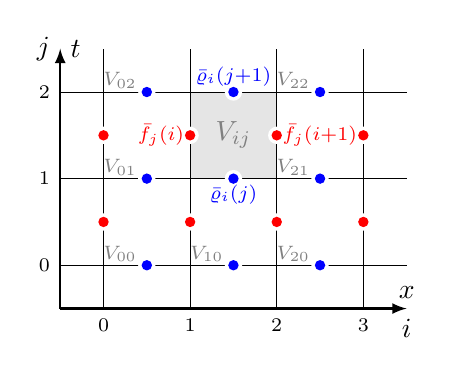
\begin{tikzpicture}[>=latex,thick,scale=1.1]

\fill[color=gray!20] (1,1) rectangle (2,2);

\def\volumen#1#2{
	\node[color=gray] at ({#1-0.12},{#2-0.08}) [above right] {$\scriptstyle V_{#1#2}$};
}

\volumen{0}{0}
\volumen{1}{0}
\volumen{2}{0}

\volumen{0}{1}
\volumen{2}{1}

\volumen{0}{2}
\volumen{2}{2}

\node[color=gray] at (1.5,1.5) {$V_{ij}$};

\foreach \x in {0,...,3}{
	\draw[line width=0.2pt] (\x,-0.5)--(\x,2.5);
	\node at (\x,-0.5) [below] {$\scriptstyle \x$};
}
\foreach \y in {0,...,2}{
	\draw[line width=0.2pt] (-0.5,\y)--(3.5,\y);
	\node at (-0.5,\y) [left] {$\scriptstyle \y$};
}
\uncover<4->{
	\foreach \x in {0,...,3}{
		\foreach \y in {0,...,1}{
			\fill[color=white] (\x,{\y+0.5}) circle[radius=0.10];
			\fill[color=red] (\x,{\y+0.5}) circle[radius=0.06];
		}
	}
	\node[color=red] at ({1+0.05},1.5)
		[left] {$\scriptstyle \bar{f}_j(i)$};
	\node[color=red] at ({2-0.05},1.5)
		[right] {$\scriptstyle \bar{f}_j(i+1)$};
}
\uncover<3->{
	\foreach \x in {0,...,2}{
		\foreach \y in {0,...,2}{
			\fill[color=white] ({\x+0.5},\y) circle[radius=0.10];
			\fill[color=blue] ({\x+0.5},\y) circle[radius=0.06];
		}
	}
	\node[color=blue] at (1.5,{2-0.05})
		[above] {$\scriptstyle \bar{\varrho}_i(j+1)$};
	\node[color=blue] at (1.5,{1+0.05})
		[below] {$\scriptstyle \bar{\varrho}_i(j)$};
}
\draw[->] (-0.5,-0.5)--(3.5,-0.5) coordinate[label={$x$}];
\node at (3.5,-0.5) [below] {$i$};
\draw[->] (-0.5,-0.5)--(-0.5,2.5) coordinate[label={right:$t$}];
\node at (-0.5,2.5) [left] {$j$};

\end{tikzpicture}
\end{center}
\vspace{-10pt}
\uncover<5->{%
\begin{block}{Differenzengleichung für $V_{ij}$}
\vspace{-15pt}
\[
\bar{\varrho}_i(j+1) - \bar{\varrho}_i(j)
=
\bar{f}_j(i+1)-\bar{f}_j(i)
\]
\end{block}}
\end{column}
\end{columns}
\end{frame}

%
% fem.tex
%
% (c) 2020 Prof Dr Andreas Müller, Hochschule Rapperswil
%
\section{Finite Elemente
\label{section:finite-elemente}}
\rhead{Finite Elemente}





